 \documentclass[12pt,a4paper]{report} %set default font to 12 and change to report

\usepackage{amsmath}
\usepackage{amssymb}
\usepackage{amsthm}
\usepackage{color}
\usepackage{algorithm}
\usepackage{algorithmic}
\usepackage{graphicx}
\usepackage{multirow}
\usepackage[title,titletoc]{appendix}
\usepackage{vector}
\usepackage{titletoc}
\usepackage{enumitem}
\usepackage{setspace} % for switching between double/single space in document
\usepackage{fancyhdr} % package for changing Headings style
\usepackage{fontspec}
\usepackage[labelsep=space,width=\hsize,format=hang,font=footnotesize,labelfont=bf]{caption}
\usepackage[labelsep=space, subrefformat=parens, width=\hsize]{subfig}
\usepackage[Kashida]{xepersian}

% این دستور به منظور تنظیم اندازهصفحه قرار داده شده است
\usepackage[paperwidth=210mm,paperheight=297mm]{geometry} %setting the page size

% setting the margins of page
\usepackage[top=2.5cm,right=3.5cm,bottom=2.5cm,left=2.5cm]{geometry}


% tell tex engine address of folder containing your pictures
\graphicspath{{images/}}

\bibliographystyle{unsrt}

\algsetup{
   linenosize=\small,
   linenodelimiter=)
}


\relpenalty=10000
\binoppenalty=10000


% تغییر و ساخت فونت های مناسب
\defpersianfont\BLotuspart[Scale=1.81]{B Lotus} % B Lotus 20
\defpersianfont\BLotussection[Scale=1.54]{B Lotus} %B Lotus 17
\defpersianfont\BLotussubsection[Scale=1.18]{B Lotus} % B Lotus 13
\defpersianfont\BLotus[Scale=1.18]{B Lotus} %B Lotus 13


% تغییر به فونت لوتوس سیاه و اندازه ی  13
\settextfont[Scale=1.18]{B Lotus} % B Lotus 13
\setsansfont[Scale=1.0]{Times New Roman}
% تغییر به فونت  11
\setlatintextfont[Scale=1.0]{Times New Roman}
\setdigitfont[Scale=1.2]{PGaramond}

% تنظیم فاصله ی بین خطوط
\renewcommand{\baselinestretch}{0.7}%setting the space between lines


\DeclareMathSizes{10}{12}{10}{8}
% -------------------------------------

\def\listfigurename{فهرست اشکال}
%\def\listtablename{فهرست جداول}
%\def\bibname{\rl{مراجع}}


\titlecontents{chapter}[1cm]
  {\bfseries\addvspace{5pt}}
  {\hspace*{-1cm}\bfseries\textsc{\chaptertitlename}\thecontentslabel-\hspace{5pt}}
  {\hspace*{-1cm}}
  {\hfill\contentspage}



\setenumerate[1]{label=\arabic*), ref=\arabic*}

\setcounter{secnumdepth}{4}
\setcounter{tocdepth}{2}

%تغییر فونت  part ها به لوتوس ساه زده شده است 
\title{\BLotuspart {گزارش جلسه سوم آزمایشگاه پایگاه داده}}%change font to b lotus 20 as defined before
\author{سامان فکری 9231075
			\and سجاد اعظمی 9231000}

\renewcommand{\contentsname}{سوالات}

\begin{document}

\Persian
\maketitle

\tableofcontents
\listoffigures
\newpage
%\listoftables

%\part{\BLotuspart{سوال 1}}%change font to b lotus 20 as defined before

%\chapter{\BLotuschapter{آشنایی با زی پرشین}}%change font to b lotus 17 as defined before


%زی‌پرشین نرم‌افزار مستقلی نیست، بلکه تنها مجموعه‌ای از ماکروها است که موتور حروف‌چینی زی‌تک با آن می‌تواند نوشته‌های فارسی را با کیفیت بسیار بالا پردازش کند.%\cite{Vapnik_1998}.

%برای نصب زی‌پرشین نخست باید یک توزیع تِک را روی رایانهٔ خود نصب کنید. منظور از یک توزیع تِک، مجموعه ای از موتورهای حروف‌چینی تک، ماکروها، قلم‌ها و ابزارهای کمکی است. معروف‌ترین توزیع‌های تک در ویندوز میک‌تک و در لینوکس تک‌لایو هستند.

%Look what happens if you put Latin text in a Persian text area.

%\Latin
%And now, this is a Latin text in a Latin text area.


%\newpage
\Persian
%\chapter{\BLotuschapter{شکل ها و جداول در زی پرشین}}%change font to b lotus 17 as defined before
%در این بخش نحوه درج جداول و شکل ها در مستندات فارسی توضیح داده میشود.




\section{\BLotussection{سوال 1}}%change font to b lotus 13 as defined before
\subsection*{\BLotussubsection{تزشیدررسیر}}
سزشرشیرشیرشیرشیریش

\begin{figure}
\caption{دماوند}
\centering
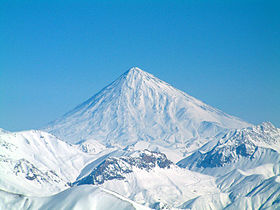
\includegraphics[height=0.3\textheight]{Damavandr.jpg}
\end{figure}



%\Latin
%\bibliography{PhdThesis}
%\begin{thebibliography}{10}

%\bibitem{Vapnik_1998}
%V.~Vapnik.
%\newblock {\em Statistical Learning Theory}.
%\newblock John Wiley \& Sons, 1998.

%\end{thebibliography}

\end{document}

